\documentclass[../main-manifolds.tex]{subfiles}

\begin{document}
\providecommand{\szz}{\mathcal{S}}
\providecommand{\ccinf}{C_c^\infty}

% Topologies
\providecommand{\Taux}{\Tau_\xx}
\providecommand{\Tauy}{\Tau_\yy}
\providecommand{\Tauxy}{\Tau_{\xx\times\yy}}

% Basis
\providecommand{\Bx}{\borel_\xx}
\providecommand{\By}{\borel_\yy}
\providecommand{\Bxy}{\borel_{\xx\times\yy}}


\fchapter{4: Submersions, Immersions and Embeddings}
\newpage

\topheader{List of Definitions}
Let $F$ be a smooth map between two smooth manifolds $M$ and $N$, with dimensions $m$ and $n$ respectively.

% Rank, constant rank, smooth submersion,, smooth immersion

\begin{definition}
    The rank of $F$ at $p\in M$ is the rank of the linear map:
\[
    dF_p: T_pM\to T_{F(p)}N
\]\end{definition}

\begin{definition}
A smooth map $F\in \cinf{M}{N}$ has constant rank if its differential $dF_p: T_pM\to T_{F(p)}N$ has the same rank at every point $p\in M$.\end{definition}

There are three types of constant rank maps that are of interest.
\begin{definition}
    $F$ is a smooth submersion if $dF_p$ is a surjection onto $T_{F(p)}N$ at $p$-everywhere. That is, $\rank dF_p = \dim T_{F(p)}N = \dim N$\end{definition}

\begin{definition}
    $F$ is a smooth immersion if $dF_p$ is an injection onto $T_{F(p)}N$ at $p$-everywhere. That is, $\rank dF_p = \dim T_{p}M = \dim M$\end{definition}

\begin{definition}
    $F$ is a smooth embedding if it is a smooth immersion, and it s a homeomorphism onto its range $F(M)\subseteq N$. 
\end{definition}

\begin{definition}
    $F$ is a local diffeomorphism if every $p\in M$ in its domain induces a neighbourhood $U\subseteq M$ with $F|U:U\to F(U)$ is a diffeomorphism (in the sense of two open sub-manifolds).
\end{definition}










\newpage
\topheader{Pre-requisites for Chapter 4}
Example 1.28 (Matrices of Full Rank)

Let $A\in\mcal({m\times n,\real})$ be the set of $m\times n$ matrices with real entries. $A$ has rank $m$ iff there exists some $m\times m$ sub-matrix of $A$, denoted by $S$ st $S$ is invertible. We wish to show the set of rank-$m$ matrices is invertible. Indeed, let 

\[
F:\mcal({m\times n,\real})\to \real,\: \Delta_{m\times m}(A) = \sum_{\mathclap{\substack{S\text{ is a } m\times m \\ \text{ sub-matrix of } A}}}|\det{S}|
\]
Since $S\mapsto \det{S}$ is continuous in the entries of $S$, hence continuous in the entries of $A$, $\Delta_{m\times m}$ is continuous.

So the set $\bigset{A\in\mcal{(m\times n,\: \real)},\: \rank{A}=m}=F^{-1}(\real\setminus\{0\})$ is open.

\newpage

Before proving the inverse function theorem, we will need several Lemmas

\begin{wts}\label{rudin-chp9-theorem-9.7}
    If $A$ and $B$ are in $L(\xx,\yy)$, then 
    \[
        \norm{BA}\leq\norm{B}\norm{A}
    \]
\end{wts}
\begin{proof}
    Let $\norm{x}=1$, and 
    \[
        \norm{B(Ax)}\leq\norm{B}\norm{Ax}\leq\norm{B}\norm{A}\norm{x}
    \]
    this holds for every $\norm{x}=1$, hence
    \[
        \norm{BA}\leq\norm{B}\norm{A}
    \]
\end{proof}
\begin{wts}\label{rudin-chp9-theorem-9.19}
    Let $f$ map a convex open set $U\subseteq\realn$ into $\realm$, if $f$ is differentiable (pointwise) in $U$, and there exists some $M$ st its derivative its founded (in the operator norm)
    \[
        \norm{Df(x)}\leq M\quad x\in U
    \]
    then, for every pair of elements $x_1$, $x_2$ in $U$,
    \[
        \norm{f(x_1)-f(x_2)}\leq M\norm{x_1-x_2}
    \]
\end{wts}
\begin{proof}
    This proof 'passes the argument' to the scalar-valued version, in short: if $x_1$ and $x_2$ are in $U$. Define
    \[
        c(t) = (1-t)x_1 + tx_2
    \]
    as the convex combination of $x_1$ and $x_2$. The takeaway intuition here is that it suffices to check on the line joining the two points', to obtain an estimate for $\norm{f(x_1)-f(x_2)}$. Indeed, define
    \[
        g(t) = f(c(t))\text{ is a curve } g:\real\to\realm
    \]
    
    Recall: Theorem 5.19
    \begin{wts}
        Let $g: [0,1]\to\realm$, and $g$ be differentiable on $(0,1)$, then there exists some $x\in (0,1)$ with
        \[
            |f(b)-f(a)|\leq (b-a)|f'(x)|
        \]
    \end{wts}
    \begin{proof}
        Read from Rudin Theorem 5.19.
    \end{proof}

    Since $Dg(t) = Df(c(t))\circ Dc(t)$ by the Chain Rule, and $Dc(t) = b-a$ by inspection,
    \[
        \norm{Dg(t)} = \norm{Df(c(t))\circ Dc(t)}\leq \norm{Df}\norm{Dc} = \norm{Df}(b-a)
    \]
    This holds for every $t\in [0,1]$. Applying Theorem 5.19 gives
    \[
        \underbrace{\norm{g(1)-g(0)}}_{\text{curve endpoints}}\leq M\norm{b-a}
    \]
    Replacing $\norm{g(1)-g(0)} = \norm{f(x_1) - f(x_2)}$ and $\norm{Df}\leq M$ we get
    \[
        \norm{f(x_1) - f(x_2)}\leq M \norm{x_1 - x_2}
    \]
\end{proof}
\newpage

Rudin Inverse Function Theorem 9.24

\begin{wts}\label{rudin-chp4-theorem-9.24}
    Suppose $f\in C^1(\realn,\realn)$, and $Df(a)$ is invertible for some $a\in\realn$, and define $b=f(a)$. Then,
\begin{enumalpha}
    \item there exist open sets $U$ and $V$ in $\realn$ such that $a\in U$, $b\in V$, and $f$ is one-to-one on $U$, and $f(U)=V$.
    \item if $g$ is the inverse of $f$ (which exists, by Part a), defined in $V$ by $g(f(x))=x$ for every $x\in U$
    then $g\in C^1(\realn,\realn)$
\end{enumalpha}
\end{wts}
\begin{proof}[Proof of Part A]
    We define $Df(a) = A\in\real^{n\times n}$, so $A$ is invertible, and $\norm{A^{-1}}\neq 0$, where $\norm{\cdot}$ denotes the operator norm. Recall all norms on finite-dimensional vector spaces are equivalent, this will be useful later.

    Choose $\lambda > 0$ st
    \begin{equation}\label{rudin-chp9-24-lambda}
        \lambda = \norm{A^{-1}}^{-1}2^{-1}
    \end{equation}

    By continuity of $Df(x)$ at the point $a$, let $\lambda > 0$, this induces a $B(\delta, a)$ with $x\in B(\delta, a)$ means

    \begin{equation}\label{rudin-chp9-24-derivative-bounded}
        \underbrace{\norm{Df(x) - Df(a)}}_{\text{operator norm}}<\lambda
    \end{equation}

    as $Df: \realn\to L(\realn,\realn)$ takes a point in $\realn$ and returns a linear map., with $L(\realn,\realn)$ endowed with the usual vector space structure. Fix $y\in \realn$, and define

    \[
        \phi(x) = \underbracket{x + A^{-1}(y}_{\text{offset}}-f(x))
    \]
    this is now a function solely in $x$, and $\phi(x)=x\iff f(x)=y$ is clear, but such a fixed point is not necessarily unique. We claim that it is unique in $B(\delta, a)$. We will use the contractive mapping principle.\\
    
    Differentiating $\phi(x)$ reads
    \[
        D\phi(x) = \underbrace{I}_{I = A^{-1}A} - A^{-1}Df(x) = A^{-1}(A-Df(x))
    \]
    \Cref{rudin-chp9-theorem-9.7} tells us the norm of a product is bounded above by the product of the norms. Using \cref{rudin-chp9-24-derivative-bounded,rudin-chp9-24-lambda}, if $x\in U$ we have
    \[
        \norm{D\phi(x)} = \norm{A^{-1}(A-Df(x))}\leq \norm{A^{-1}}\norm{A-Df(x)}\leq 2^{-1}
    \]
    The total derivative of $\phi$ is uniformly bounded in $U$, applying \Cref{rudin-chp9-theorem-9.19} tells us that $\phi$ is a contractive mapping
    \[
        \norm{D\phi(x)}\leq 2^{-1}\implies \norm{\phi(x_1)-\phi(x_2)}\leq 2^{-1}\norm{x_1-x_2}
    \]
    for $x_1$, $x_2$ in $U$.\\

    To show $f|U$ is indeed a bijection, fix $y\in f(U)$ so $y = f(x)$ for some $x\in U$, and there can only be one fixed point stemming from $\phi|U$, with $\phi(z) = z + A^{-1}(y-f(z))$ being the 'fixed point detector'. Write $(f|U)^{-1}(y) = \lim \{(\phi|U)(x_n)\}_n$ and every point in $f(U)$ has a unique inverse.\\

    For the last part of the proof, we wish to show $V = f(U)$ is open. Let $y_0\in V$ and we can 'hone into' the inverse of $y_0$ using the same construction as earlier. So $f(x_0) = y_0$ for some unique $x_0\in U$.\\
    
    If $x_0$ is in $U$, it induces an open ball (see \cref{rudin-chp9-open set induces ball that hides inside}) st
    \[
        x_0\in B(r,x_0)\subseteq \cl{B(r,x_0)}\subseteq U,\quad r>0
    \]

    \begin{figure}
        \centering
        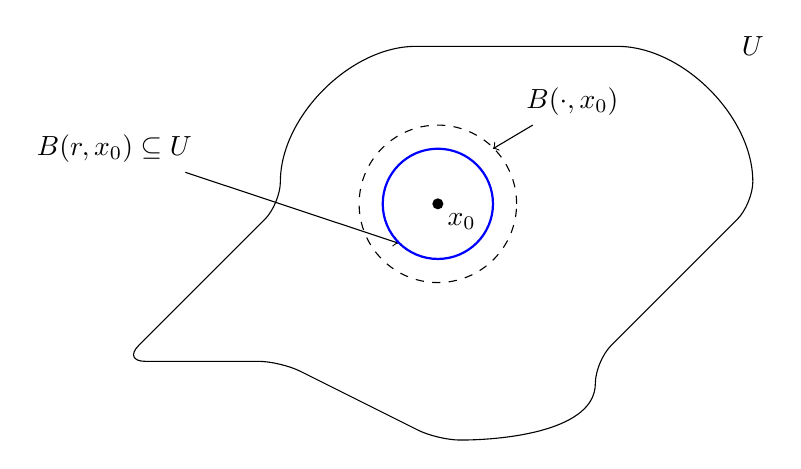
\begin{tikzpicture}
        % Draw the open set U
        \draw[rounded corners=8pt] (0,0) -- (2,2) to[out=90,in=180] (4,4) -- (6,4) to[out=0,in=90] (8,2) -- (6,0) to[out=-90,in=0] (4,-1) -- (2,0) -- cycle;

        % Label the set U
        \node at (8,4) {$U$};

        % Draw the point x
        \fill (4,2) circle (2pt);
        \node[below right] at (4,2) {$x_0$};

        % Label
        \node[above right] at (5,3) (ball) {$B(\cdot, x_0)$};
        \draw[->] (ball) -- (4.7,2.7);

        \node[below left] at (1,3) (ball) {$\cl{B(r, x_0)}\subseteq U$};
        \draw[->] (ball) -- (3.5 ,1.5);

        % Draw the open ball around x
        \draw[dashed] (4,2) circle (1);
        \draw[thick, blue] (4,2) circle (0.7);
        \end{tikzpicture}
        \caption{Every point $x_0$ in an open set $U$ admits an open ball that hides in $U$}
        \label{rudin-chp9-open set induces ball that hides inside}
    \end{figure}

    We claim the open ball $B(\lambda r, y_0)\subseteq V$. Indeed, suppose $y\in\realn$ with 
    \[
        d(y,y_0) < \lambda r
    \]
    If $\phi$ is the 'fixed-point detector' with respect to $y$ (the point we are trying to prove that is in $f(U)$), in fact: we will prove $y\in f(\cl{B(r,x_0)})\subseteq f(U)$.
    \[
        \underbracket{\phi(x_0) - x_0}_{\text{removing the offset from }\phi(x_0)} = A^{-1}(y - f(x_0)) = A^{-1}(y - y_0)
    \]
    using the operator norm on $A^{-1}(y-y_0)$ reads
    \[
        \norm{\phi(x_0) - x_0} = \norm{A^{-1}(y-y_0)}\leq \norm{A^{-1}}\norm{y-y_0}\leq \norm{A^{-1}}\lambda r = r2^{-1}
    \]
    We will drag $y$ into the image of the closed ball as follows: suppose $x$ is another point that lies in the closed ball, $\phi$ is contractive on $\cl{B}\subseteq U$ regardless of the point $y$ that induces $\phi$. But $\cl{B}$ is closed, hence it is complete. So the Cauchy sequence (from the contractive mapping theorem) produces exactly one point in $\cl{B}$. It remains to show that if we start our sequence at some point $x\in \cl{B}$, then $\phi(x)\in\cl{B}$ as well, and a simple induction will produce our contractive sequence.\\


    To this, fix $x\in \cl{B}$, and 
    \begin{align*}
        |\phi(x)-x_0|&\leq |\phi(x)-\phi(x_0)| + |\phi(x_0)-x_0|\\[1ex]
        &\leq \overbracket{2^{-1}|x-x_0|}^{\text{contraction on } \cl{B}\subseteq U} + \overbracket{r2^{-1}}^{\text{earlier}} \\[1ex]
        &= r
    \end{align*}
    therefore $\phi$ contracts to a fixed point $x^*\in \cl{B}$, and $f(x^*)=y$. So $y\in f(\cl{B})\subseteq f(U)$ as desired.
\end{proof}
\begin{proof}[Proof of Part B]
    The proof is quite long, and we will only focus on the important bits. Rudin uses the technique of approximating smooth functions using first-order terms. He writes
    \[
        \begin{cases}
            f(x) &= y \\
            f(x+h) &= y+k
        \end{cases}
        \implies k = f(x+h) - f(x)
    \]
    Furthermore, if $x\in U$, then the derivative $Df(x)$ is invertible, this is from Theorem 9.8, obtains an estimate on the open ball in $GL(n,\real)$. Roughly speaking, this open ball 'drags' other matrices into $GL(n,\real)$. If $A$ is invertible, and $B$ is a conformable matrix with $A$, then
    \[
    \underbracket{\norm{B-A}}_{\substack{\text{distance} \\ \text{between}\\ A, B}}\norm{A^{-1}}<1\implies B\in GL(n,\real)
    \]
    If $x\in B(\delta, a)$, then \Cref{rudin-chp9-24-derivative-bounded} reads 
    \[
        \norm{Df(x) - A}<\lambda\implies \norm{Df(x) - A}\norm{A^{-1}}<2^{-1}<1
    \]
    so $Df(x)$ is invertible with inverse $T$.\\

    And we estimate the deviation $|k|^{-1}\leq \lambda|h|^{-1}$ by using the contraction inequality with $y$ as the basepoint for $\phi$. Skipping a few lines ahead (to the confusing part), we see that
    \[
        |h|\leq |h-A^{-1}k| + |A^{-1}k|\leq 2^{-1}|h| + |A^{-1}k|
    \]
    subtracting over, and multiplying across gives a upper bound on $|k|^{-1}$
    \[
        2^{-1}|h|\leq |A^{-1}k|\implies 2^{-1}|h|\leq\norm{A^{-1}}|k|\implies |k|^{-1}\leq \underbracket{\dfrac{2}{\norm{A^{-1}}}}_{\lambda}|h|^{-1}
    \]
    Notice $2\lambda\norm{A^{-1}}=1$, so $2/\norm{A^{-1}}=\lambda$. Finally, we 'factor out' $-T$ on the line just before the difference quotient.
    \begin{align*}
        \overbracket{g(y+k)-g(y) - Tk}^{\substack{\text{numerator in }\\ \text{difference quotient}}} &= h - Tk \\[1ex]
        &= -T\biggl(\underbracket{f(x+h) - f(x)}_{=k} - \underbracket{Df(x)h}_{=T^{-1}h}\biggr)
    \end{align*}
    We see that $T = Dg(y)$, indeed:
    \begin{align*}
        \dfrac{|g(y+k)-g(y)- Tk|}{|k|}&\leq\dfrac{\norm{T}}{\lambda}\dfrac{|f(x+h)-f(x)-Df(x)h|}{|h|}\\
        &\Lsim \dfrac{|f(x+h)-f(x)-Df(x)h|}{|h|} \\
        = \underbracket{o(h) = o(k)}_{|h|\Lsim |k|}\to 0
\end{align*}

Finally, $Df|U: U\to GL(n,\real)$ is a continuous mapping. By Theorem 9.8, $(Df|U)^{-1}: U\to GL(n,\real)$ is continuous as well. Therefore $g\in C^1(U,U)$, and $f|U$ is a $C^1$-diffeomorphism.
\end{proof}

\newpage

\topheader{Commentary}

Proposition 4.1 roughly states that, if the differential of $F$ at some point $p$ is injective or surjective, then there exists a neighbourhood $U$ about $p$ such that $dF|U(p)$ is an injection or surjection. The continuity of the map $dF|U(p) \mapsto \Delta_{m\times m}(dF|U(p))$, induces a neighbourhood in the vector space of matrices about the differential $dF|U(p)$. This vector space is endowed with any of the equivalent norms on $\mcal(m\times n,\real)$, which is equivalent to the entrywise $2$-norm. Since all partials of the form $\eval{\pdv{\hat{F}^{k}}{x^j}}_{\hat{p}}$ are continuous, we take the intersection over all $n\times m$ partials such that $dF|U(p)$ is an injection or surjection. Finally, send this neighbourhood about $\hat{p}$ through to $p$ by using the continuity of $\phi$.



\end{document}